Desenvolva um projeto que realize a comunicação entre dois microcontroladores utilizando o padrão SPI.

\section{O que é o Padrão SPI?}

Neste trabalho iremos mostrar uma das diversas tecnologias diferentes existentes para fazer a comunicação serial entre dois dispositivos. Durante o discorrer deste estaremos trabalhando com o padrão \sigla{SPI}{Serial Peripheral Interface}.

Na comunicação serial síncrona definimos também o conceito de Mestre-Escravo. Normalmente o gerador do sinal de sincronismo é definido como o Mestre (Master) da comunicação. Para os dispositivos que utilizam do sinal de sincronismo gerado damos a definição de Escravo (Slave). A ligação mais comum desse tipo de comunicação é um Master e vários Slaves.

\begin{figure}[htb]
 \caption{Master and Slaves}
 \label{fig:Master and Slaves}
 \centering
 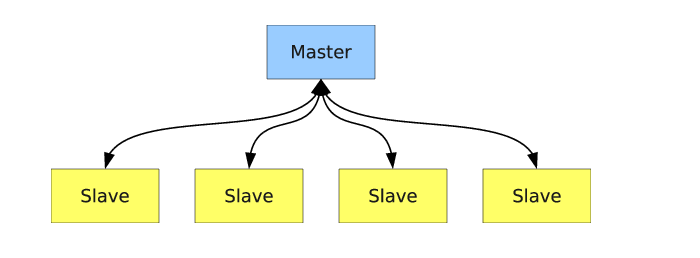
\includegraphics[scale=0.5]{Master_And_Slave.png}
 \fdireta{embarcados:master_slave}
\end{figure}

Os pinos básicos de comunicação entre dispositivos utilizando o protocolo SPI e o esquema padrão de ligação são dados conforme abaixo:

\begin{figure}[htb]
 \caption{Pinos do SPI}
 \label{fig:Pinos para comunicação SPI}
 \centering
 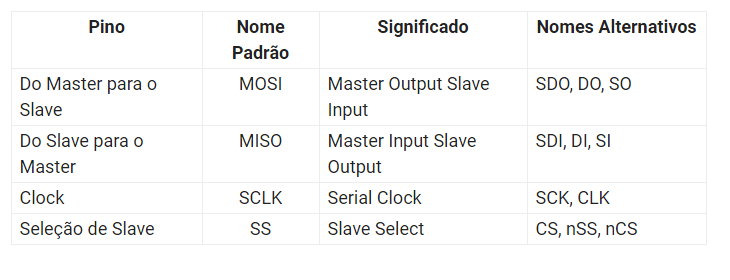
\includegraphics[scale=0.5]{pinos.png}
 \fdireta{embarcados:master_slave}
\end{figure}

O sinal de SS funciona como Seleção de Escravo (Slave Select). É um sinal ativo em nível baixo, o que significa que o dispositivo é selecionado quando este pino se encontra em nível baixo. No entanto, muitos dispositivos utilizam este sinal como sincronismo de frame. Dessa forma, é um sinal importante que deve ser respeitado.

\section{Esquemático e Montagem}

Neste projeto realizaremos a comunicação entre dois microcontroladores distintos com o uso do padrão \sigla{SPI}{Serial Peripheral Interface}, que trata-se de um protocolo que permite a comunicação de um microcontrolador com diversos outros componentes, formando uma rede. Os dois microcontroladores utilizados serão identificados por mestre e escravo (master / slave). O mestre será encarregado de enviar os comandos através da comunicação serial, enquanto o escravo é encarregado de receber, interpretar e executar uma determinada ação com base nos dados recebidos. Os comandos enviados de um microcontrolador são um indicador de qual será o estado de um LED, ligado ou desligado.

Veja o esqumático na imagem abaixo: 

\begin{figure}[htb]
 \caption{SPI: Esquemático da montagem}
 \label{fig:SPI: Esquemático da montagem}
 \centering
 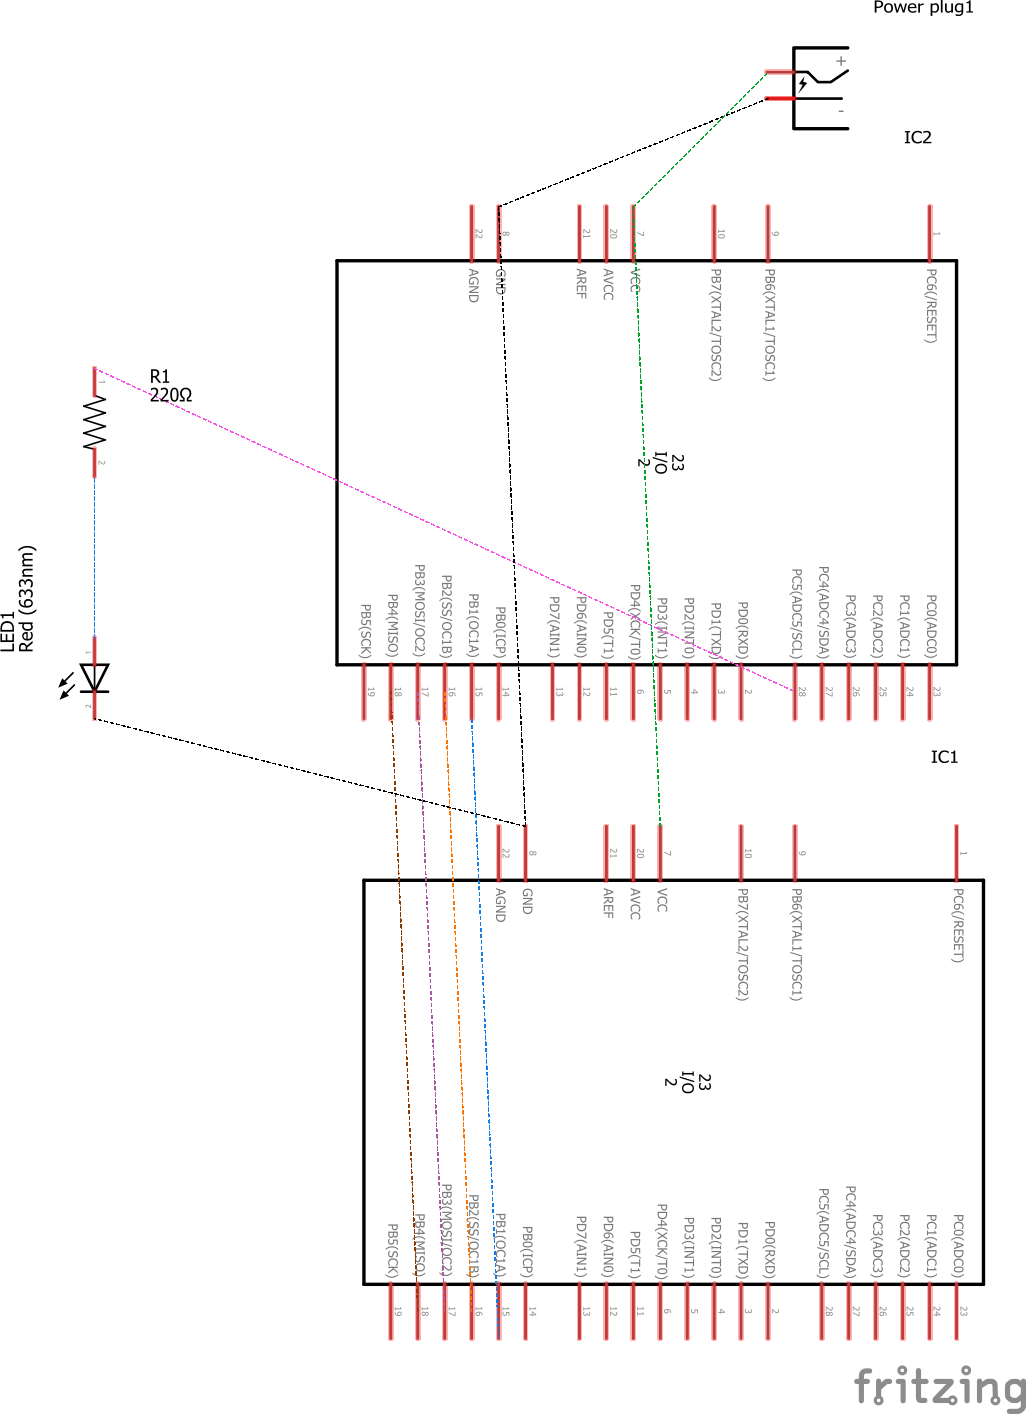
\includegraphics[scale=0.5]{SPI_esquematico.png}
 \fautor
\end{figure}

\begin{figure}[htb]
 \caption{SPI: Montagem na Protoboard}
 \label{fig:SPI: Montagem na Protoboard}
 \centering
 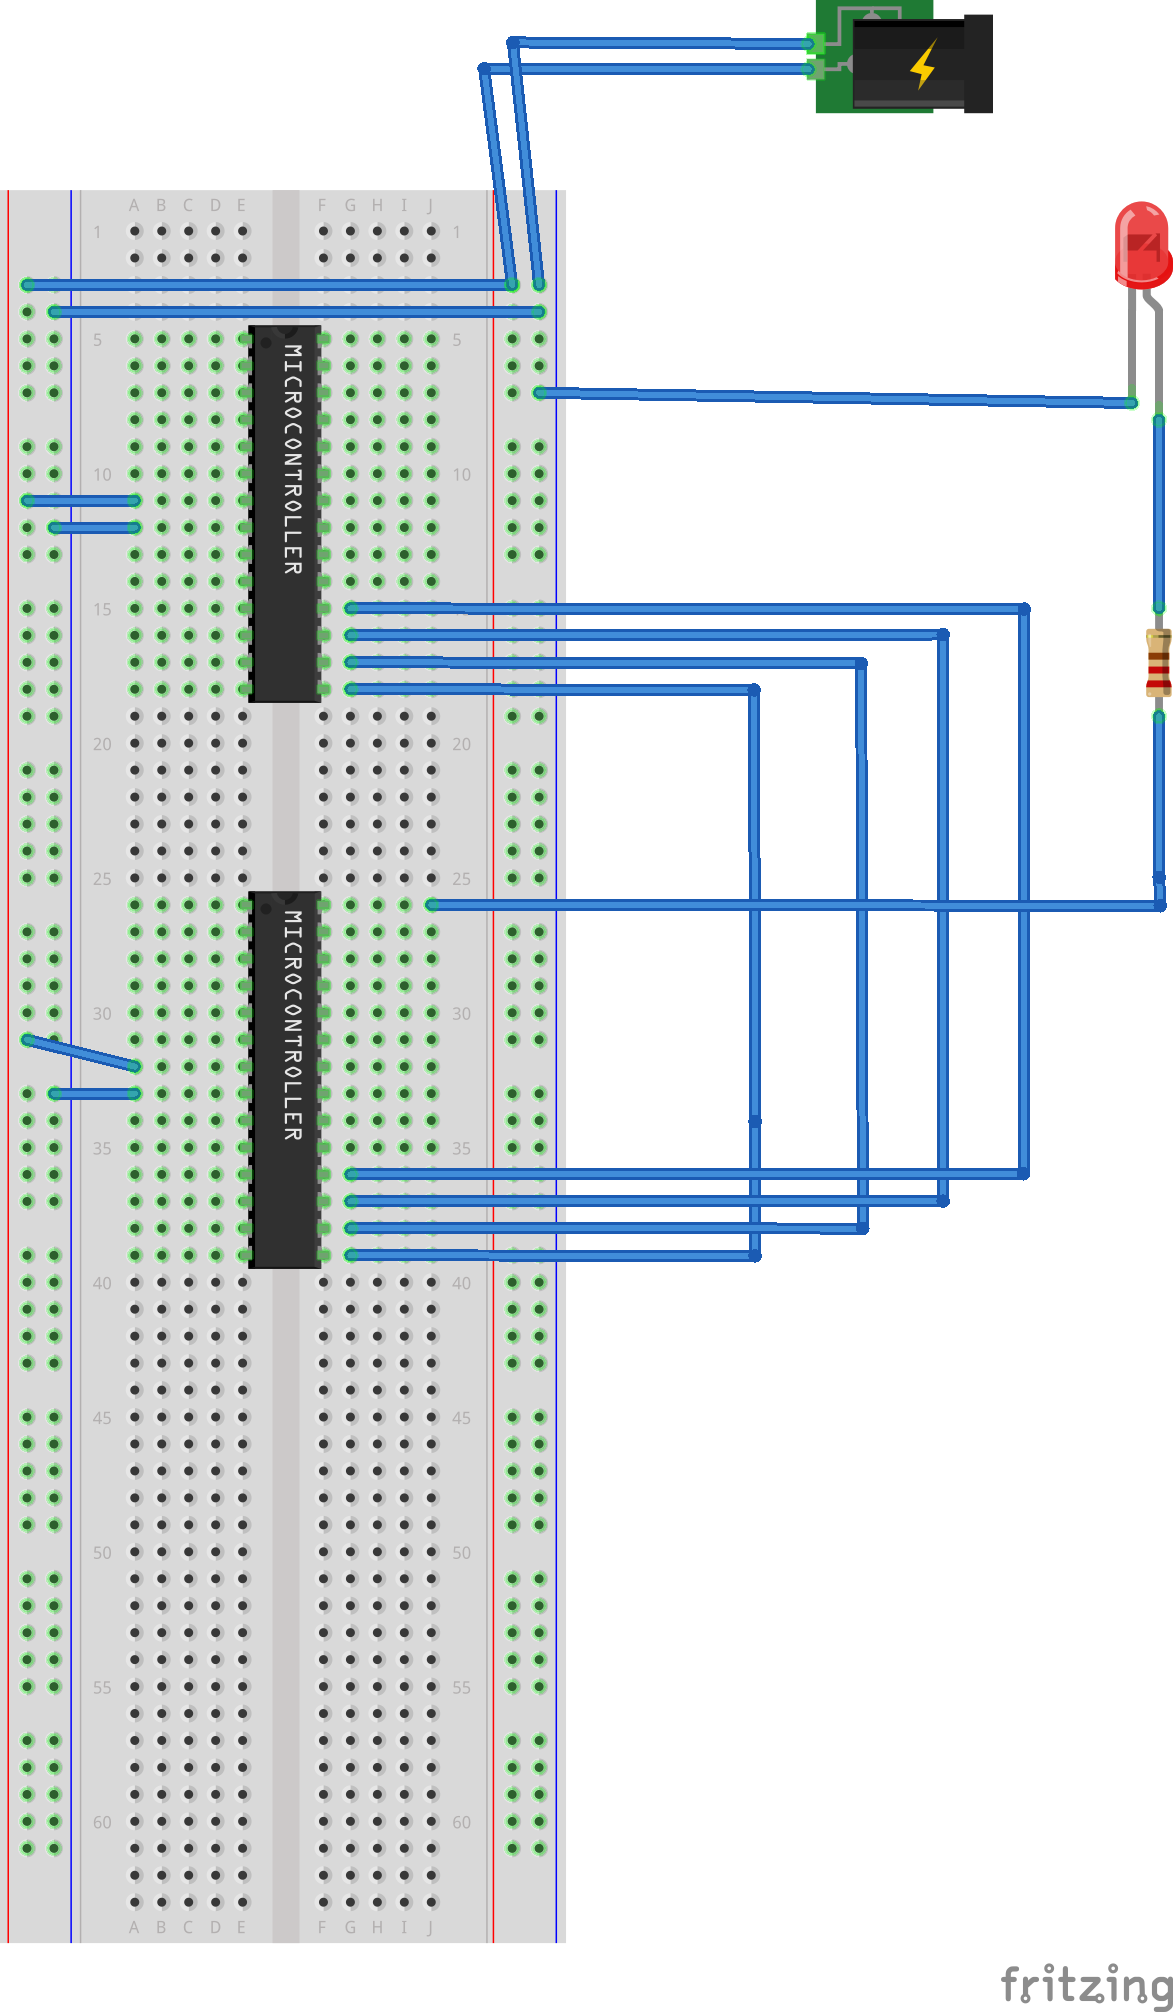
\includegraphics[scale=0.5]{SPI_montagem.png}
 \fautor
\end{figure}

\section{Código em C}

O código para este projeto é dividio em duas partes: Código do Master e o Código do Slave.

\begin{codigo}[caption = {MASTER - Comunicação via SPI entre dois dispositivos}, label={codigo: Comunicação entre dispositivos AVR usando SPI - MASTER },language=C, breaklines=true]

 /**************************************************************************
 *      Comununicação entre dois Microcontroladores Utilizando  SPI (Master)
 *
 * Universidade Federal de Goiás
 * Microcontrolador Utilizado: AVR ATMega8
 * Grupo: Marco Túlio / Vitor do Vale Bernardo / Pablo Silva
 * Descrição: Codigo Master irá enviar comandos pela comunicação SPI para o slave
 *            O comando ira dizer o estado do LED: ligado ou desligado.
 * 
 ************************************************************************/
    

#define F_CPU 4000000UL           // clock do microcontrolador
#include <avr/io.h>
#include <util/delay.h>
#include <avr/interrupt.h>
 
/////////////////////////////configuração dos pinos utilizados //////////////////////////////////////
 
#define MOSI         PB3
#define MISO         PB4
#define SCK          PB5
#define SS           PB2
 
/////////////////////////////////////////////////////////////////////////////////////////////////////////
  void SPI_inicializa(void)
  {
      DDRD =0xFF;
      DDRB |= ((1<<MOSI)|(1<<SCK)|(1<<SS));    //MOSI, SCK and SS são saidas(se for usar dois mestres então deve-se o SS como entrada) 
      DDRB &= (~(1<<MISO));                    //MISO é entrada
      PORTB |= (1<<SS);                        //inicia com SS em nivel alto
      //SPE : habilita SPI
      //MSTR: modo  Master 
      //SPIE:  habilita interrupção de SPI
      //SPCR = ((1<<SPE)|(1<<MSTR)|(1<SPR1)|(1<SPR0));    //(1<SPR1)|(1<SPR0) : FOSC/128
      SPCR = ((1<<SPE)|(1<<MSTR)|(1<SPR0));    //(1<SPR0) : FOSC/16
  }
   
  void SPI_envia_byte(char dados)
  {
      PORTB &= (~(1<<SS));    //coloca SS em nivel baixo (0), para transferir dados
      SPDR = dados;        //inicializa transferencia
      while(!(SPSR & (1<<SPIF)));    //espera fim de transmissão
      PORTD = SPDR;//escreve no port D o dado recebido
      PORTB |= (1<<SS);    //coloca SS em nivel alto (1), pois é o fim da transmissão.
      _delay_ms(1);//tempo para slave colocar dados no registrador
  }
   
  int main(void) 
  {
    
    SPI_inicializa();//inicializa SPI
    sei();//habilita interrupções
   
    while(1)
	{
      SPI_envia_byte(0X01); /*** Envia o primeiro comando: LIGAR LED***/
      _delay_ms(1000); /*** Delay de 1 segundo ***/
	   SPI_envia_byte(0x00); /*** Envia o segundo comando: DESLIGAR LED ***/
	   _delay_ms(1000);  /*** Delay de 1 segundo ***/
  }
   
    return 0;
  }

\end{codigo}


\begin{codigo}[caption = {SLAVE - Comunicação via SPI entre dois dispositivos}, label={codigo: Comunicação entre dispositivos AVR usando SPI - SLAVE },language=C, breaklines=true]

 
 /**************************************************************************
 *      Comununicação entre dois Microcontroladores Utilizando  SPI (Slave)
 *
 * Universidade Federal de Goiás
 * Microcontrolador Utilizado: AVR ATMega8
 * Grupo: Marco Túlio / Vitor do Vale Bernardo / Pablo Silva
 * Descrição: Codigo Slave irá receber os dados enviados pelo Master e colocara no PORTD,
 *            Ligando e desligando o LED.
 * 
 ************************************************************************/
    
   #define F_CPU 4000000UL  // Definindo o Clock do Microcontrolador
   #include <avr/io.h>
   #include <avr/interrupt.h>
   
   /*********************************
   *	Definindo os Registradores  *
   *********************************/
   
   #define MOSI     PINB3 /*******Definindo o PINB3 como entrada********/
   #define MISO     PINB4 /********Definindo o PINB4 como saída********/
   #define SCK      PINB5 /********Definindo o PINB5 como entrada********/
   #define DDR_SPI  DDRB
    
   char enviar=0;
    
   /*********************************
   *	Inicializando			    *
   *********************************/
   
   void SPI_Slave_inicializa(void)
   {
       DDR_SPI = (1<<MISO);
       SPCR = (1<<SPE)/*|(1<<CPOL)*/|(1<<SPIE); /****Aviva o SPI / polaridade do clock / habilita interrupção de SPI ****/
   }
   
   /**** Vetor de Interrupção *****/
   ISR (SPI_STC_vect)                         
   {
     SPDR = enviar; //envia dado anteriormente recebido
     PORTD = SPDR;
	 PORTC = SPDR;
     enviar = SPDR;
   }
   
   /*********************************
   *	Função Principal		    *
   *********************************/
   int main(void) 
   { 
       SPI_Slave_inicializa();
       DDRD = 0xFF;
       DDRC = 0XFF;
	   sei();
	   
	   while(1){
		   
	   }

   }

\end{codigo}


















